\chapter[Cryo-ET and STA]{Cryo-electron tomography and subtomogram averaging}\label{et}

Compared to X-ray crystallography, SPA sample preparation is a strong selling point: it can be much faster and simpler, not requiring crystallization and needing small quantities of sample, and being less sensitive to contamination.
Thanks to the fast vitrification, SPA is also better for studying the sample at near-native state, and for capturing rare or dynamic states (though the analysis in these cases becomes trickier).
However, due to the unknown particle orientations and low SNR, SPA data analysis is trickier and more error-prone, especially for small particles (\lesssim100 kDa), where X-ray crystallography is usually the better choice.

On the other hand, bigger particles or complexes are usually better handled by cryo-EM: with larger molecular size, crystallization gets increasingly difficult, and NMR can no longer be effectively used for structural determination.
On the other hand, NMR allows to gather some information on the dynamics of the sample, even large ones and even directly in solution, since there's no need for crystallization or vitrification.
This, however, requires appropriate isotope or methyl labeling and very high concentrations, which may cause aggregation or non-native conformations.

All these techniques rely on drawing information about an ensemble of molecules, typically with a purified sample prepared \textit{in vitro}.
However, macromolecular systems can often be fully understood only by accounting for their biological context, which is partly or fully lost in the expression and purification process.
When studying biological systems that form larger, heterogenous mesoscale complexes --- spanning hundreds of nanometers, often called superstructures --- having a three-dimensional understanding of individual events within their cellular context becomes paramount.

While ML tools such as AlphaFold3~\cite{abramsonAccurateStructurePrediction2024} have recently become powerful enough to accurately predict even large protein complexes, they still suffer from the same decontextualization problem as all these experimental techniques.

A method that promises to solve these problems is cryo-electron tomography (cryo-ET): a technique that can look not only at purified macromolecules, but at entire cells and tissues, \textit{in situ} in near-native conditions, with the ability to reach higher resolutions via subtomogram averaging, while retaining contextual information and providing a 3D view into single events.

Tomographic reconstruction is not a recent invention: the first appearance goes back more than a century~\cite{jDeterminationFunctionsTheir1917}; its successful application to cryo-EM, however, is only a recent development closely linked to the resolution revolution, which allowed to finally overcome the biggest overarching limitation of cryo-ET --- poor signal-to-noise ratio --- enough to reach sub-nanometer resolutions~\cite{lucicCryoelectronTomographyChallenge2013,turkPromiseChallengesCryoelectron2020}.

At its core, cryo-ET is just cryo-EM with extra steps; they share much of the theory, hardware and software.
The key difference is that, where single particle cryo-EM uses projections from different \textit{copies} of the same object to reconstruct a 3D map, cryo-ET images the same location from multiple orientations in order to reconstruct a 3D map from multiple projections of the \textit{same} object.
This section describes the theory of cryo-ET, how it deviates from SPA, and the current state of the art with its limitations and upcoming developments.

\localtableofcontents

\section{Sample preparation}
As with SPA, vitrification remains the key step of sample preparation for cryo-ET.
Due to the intrinsically worse SNR --- caused by the lower electron dose used during data collection, necessary to preserve the sample (\fullref{et_data_collection}) --- cryo-ET sample preparation requires extra care to reduce any possible source of additional noise.

One such source is the thickness of the sample; while this problem can be avoided by preparing thinner model systems \textit{in vitro}, it's otherwise unavoidable for samples such as entire cells or organelles, where the \textit{in situ} benefits of cryo-ET really shine.
A thick sample poses also another problem: with thickness higher than a few μm (most mammalian cells), plunge freezing does not have a fast enough cooling rate to prevent the formation of crystalline ice.
For these reasons, a combination of two techniques is often used: high-pressure freezing (HPF) and cryo-ultramicrotomy.
In HPF, the sample is put under great pressure (>200 MPa) before ultrarapid freezing, preventing expansion and thus lowering the cooling rate needed for vitrification, without the need for potentially cell-disrupting cryoprotectant~\cite{moorInfluenceHighPressure1980,bergerCryoelectronTomographyFocused2023}.
Then, cryo-ultramicrotomy uses a diamond knife to cut from the sample very thin slices, that are then deposited on a grid for imaging~\cite{peaseElectronMicroscopyUltramicrotomy1981}.
In recent years, focused ion beam (FIB) milling --- a technique already well established in material sciences --- has found widespread use in cryo-ET sample preparation, allowing to slice thin lamellae from a vitrified sample without incurring in the shear and surface deformations of cryo-ultramicrotomy~\cite{markoFocusedionbeamThinningFrozenhydrated2007}.

\subsection{FIB milling}
FIB milling typically makes use of a gallium ion beam --- or, more recently, xenon or oxygen plasma --- to ablate thick samples, which can be thus thinned to below 150 nm.
Preparing lamellae via FIB milling is becoming standard procedure in cryo-ET, and many cryo-ET facilities are automating much of the process, increasing reliability, speed and reproducibility.

\begin{figure}[ht]
    \centering
    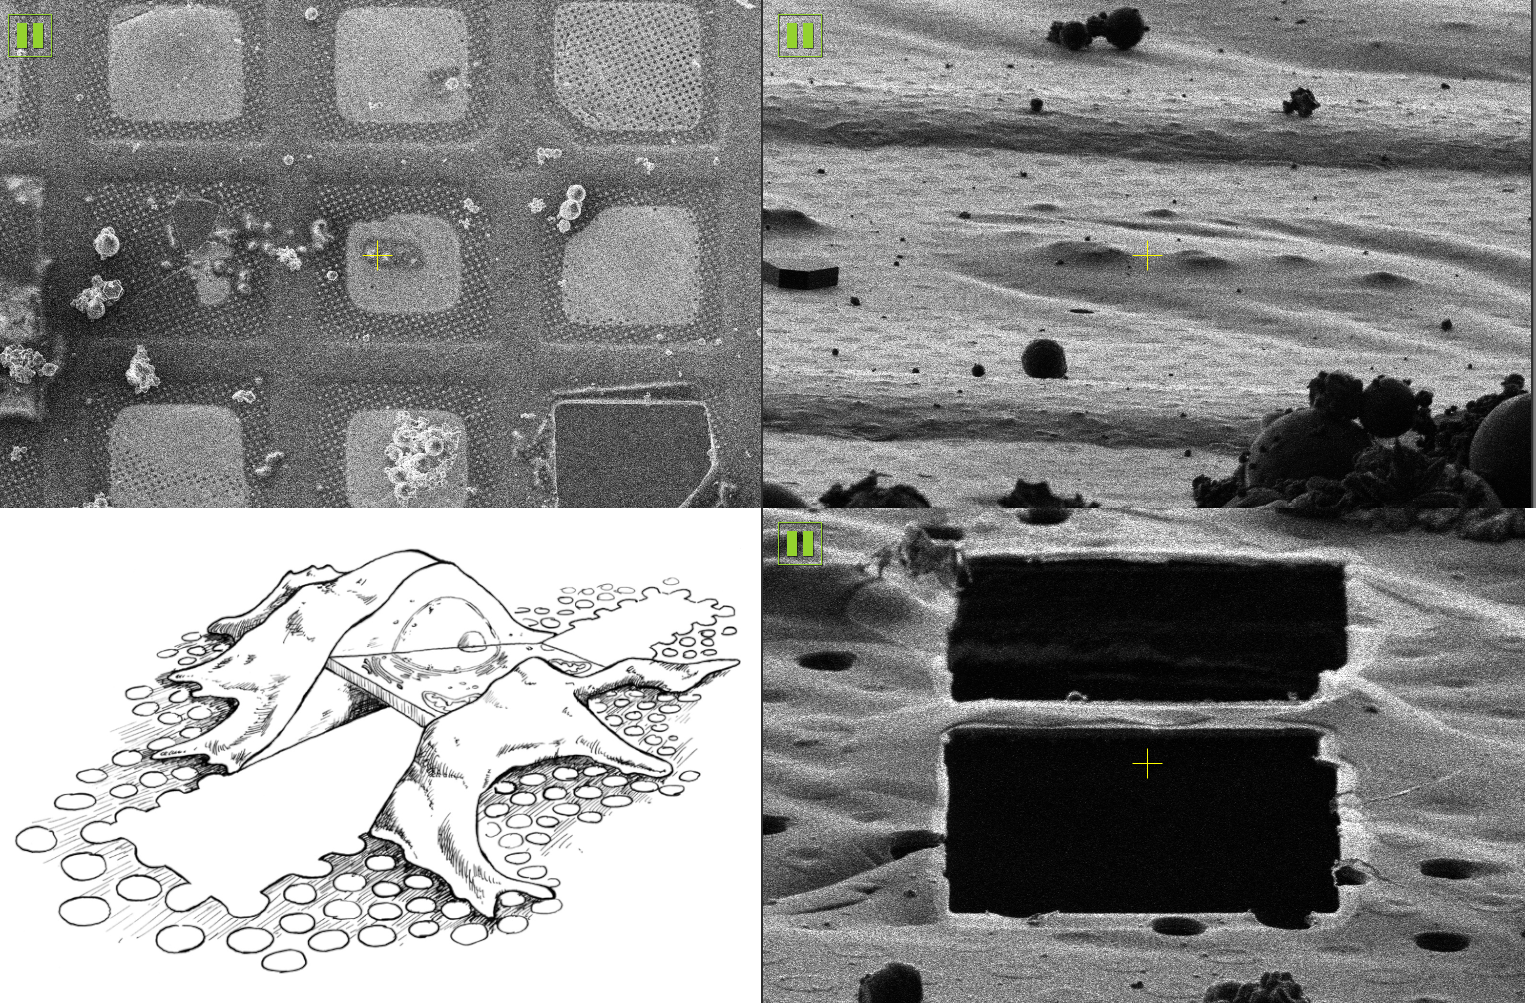
\includegraphics[width=\textwidth]{introduction/fib.png}
    \titledcaption[FIB milling]{Microscope snapshots from FIB milling procedure on \textit{Deinococcus radiodurans}. A cluster of cells, visible as a bump on the SEM, is selected from the grid (top left). From a shallow angle of around 15° from the grid (top right) the FIB is used to ablate material above and below the area of interest. This leaves a thin lamellae suitable for cryo-ET (bottom). Milled cell drawing (bottom left) taken from \citet{villaOpeningWindowsCell2013}.}
    \label{fig:et_fib_milling}
\end{figure}

% TODO: CLEM perspectives? where to put?

\subsection{Fiducials}\label{fiducials}
During data collection, despite vitrification, samples undergo different kinds of deformations.
Moreover, due to the intrinsic imprecision of controlling the hardware of the microscope, there will always be some shift and angle mismatch between different tilts during a tilt series collection (\fullref{et_data_collection}).

To help with correcting these errors, it is often useful to add to the sample some fiducials: small high-contrast, round objects (typically 10 nm gold beads) that can be easily located in the images and later used to estimate sample shift, rotation, and deformations (\fullref{et_tilt_series_alignment}).

\section{Data collection}\label{et_data_collection}
In order to acquire a sequence of images at different tilts (termed \textbf{tilt series}) for tomographic reconstruction, the same area of the sample needs to be imaged multiple times, at a range of different angles.
During collection, the sample is rotated around a tilt axis perpendicular to the electron beam, in small angular increments so as to expose a different view to the electron beam.
It's important to position the sample at \textbf{eucentric height} --- the height at which a rotation of the sample no change in focus nor a lateral movement --- so that the area of interest remains at the same focus and at the center of the field of view.

Due to the multiple exposures, in order to preserve the specimen from radiation damage the electron dose must be fractionated to much lower than typical in SPA, but still high enough to capture enough signal to allow motion correction~\cite{mcewenRelevanceDosefractionationTomography1995}.

Each subsequent exposure further damages the sample, which degrades the high resolution information first.
This, in combination with the fact that in cryo-ET the electron beam has to traverse a thicker sample at high tilts --- leading to worse SNR --- created the need for optimized collection schemes.
The most commonly used nowadays is the Hagen (or dose-symmetric)  scheme~\cite{hagenImplementationCryoelectronTomography2017}: it collects the first image at 0° tilt, and then alternates between negative and positive tilts until it reaches the maximum tilt.
This minimizes the radiation damage when SNR is best, allowing to capture high resolution information at its prime, before it is degraded by cumulative exposures.

Due to the geometry of the sample and its support within the microscope, there is a limit to how high an angle can be reached when tilting the sample.
This angle is typically around 60-70°, beyond which the sample becomes too thick for imaging at such low doses, and the grid bars come into view obscuring part of the sample.
This will result in a \textbf{missing wedge} of information in Fourier space during tomographic reconstruction (\fullref{et_tomo_reconstruction}).

Conventional wisdom sets the interval between subsequent tilts at around 3° to ensure enough fourier space filling while limiting radiation damage, though depending on the application --- especially where certain spatial frequencies are considered important or over-represented in the sample --- it might be worth considering smaller, wider, or non-linear increments~\cite{copeCryoElectronTomographyStructural2011}.

\section{Preprocessing}
Cryo-ET data undergoes similar preprocessing steps as SPA data (\fullref{em_preprocessing}), albeit with less precision due to the low electron dose.

While at this point single particle data is ready for particle picking and other downstream work, cryo-ET data must still undergo tomographic reconstruction in order to obtain the 3D volumetric reconstruction of the sample.

To do so, tilt series alignment parameters must first be estimated in order to correct for equipment imprecision and sample deformations, and then used for 3D volume reconstruction.

\subsection{Tilt series alignment}\label{et_tilt_series_alignment}
The most basic alignment procedures require at least full-frame aligment; similar to motion correction, tilt images are rotated and shifted in order to maximize their CC score.
Where fiducials are present (\fullref{fiducials}), these can be treated as static points within the sample and used instead as anchors to mathematically estimate the geometric transformation between different tilts~\cite{nicastroMolecularArchitectureAxonemes2006,heumannClusteringVarianceMaps2011,castano-diezDynamoCatalogueGeometrical2017}.

In state of the art software, alignment procedures (with or without fiducials) can also account for spatio-temporal deformations of the sample, either already during tilt series alignment~\cite{zhengAreTomoIntegratedSoftware2022}, or later during refinement~\cite{tegunovMultiparticleCryoEMRefinement2021,burtImageProcessingPipeline2024,galaz-montoyaSingleParticleTomography2015,chenCompleteDataProcessing2019} (\fullref{et_refinement}).

\subsection{Tomogram Reconstruction}\label{et_tomo_reconstruction}
Similarly to how 3D reconstructions are obtained from 2D particles in SPA based on the central slice theorem (\fullref{em_reconstruction}), the aligned tilt series can be used to reconstruct the full tomogram.
Depending on the software suite and workflow, full tomogram reconstructions may be used only for template matching (\fullref{et_particle_picking}) and segmentation purposes, or also to extract subtomograms at small pixel sizes for subtromogram averaging (\fullref{et_sta}).

Differently from SPA, cryo-ET has the advantage of knowing the 3D positioning of features in the tomogram.
This allows to bring defocus estimation and CTF correction to the next level: not only is CTF locally estimated depending on the in-plane position of features, but also accounting for the defocus difference between the top and bottom of the sample.
While this idea was around for a long time, only in recent years tools were developed that can run in reasonable time and significantly improve the final resolution~\cite{turonovaEfficient3DCTFCorrection2017,tegunovRealtimeCryoelectronMicroscopy2019}. 
Depending on the software, 3D-CTF might be estimated and corrected at different levels (tilt image, full tomogram or subtomogram), and may be able to be refined during refinement (\fullref{et_refinement}).

Due to the limited range of tilt angles collected in typical cryo-ET workflows, not all views of the sample are represented; when reconstructing the 3D FT of the sample, this is clearly visible in fourier space as a wedge of missing information (\autoref{fig:et_missing_wedge}).
The missing wedge introduces several problems in downstream processing: it blurs the tomogram in the Z direction, biases subtomogram alignment, and leads to anisotropic resolution for objects with preferential orientation.

If fiducials (or other high-contrast objects of no real interest) are present in the sample, it is often useful to mask them during reconstruction, in order to avoid the high-contrast artifactual streaks caused by the missing wedge, which can impair the interpretability of the tomogram~\cite{tegunovRealtimeCryoelectronMicroscopy2019,burtTeamtomoFidder2024}.

\begin{figure}[ht]
    \centering
    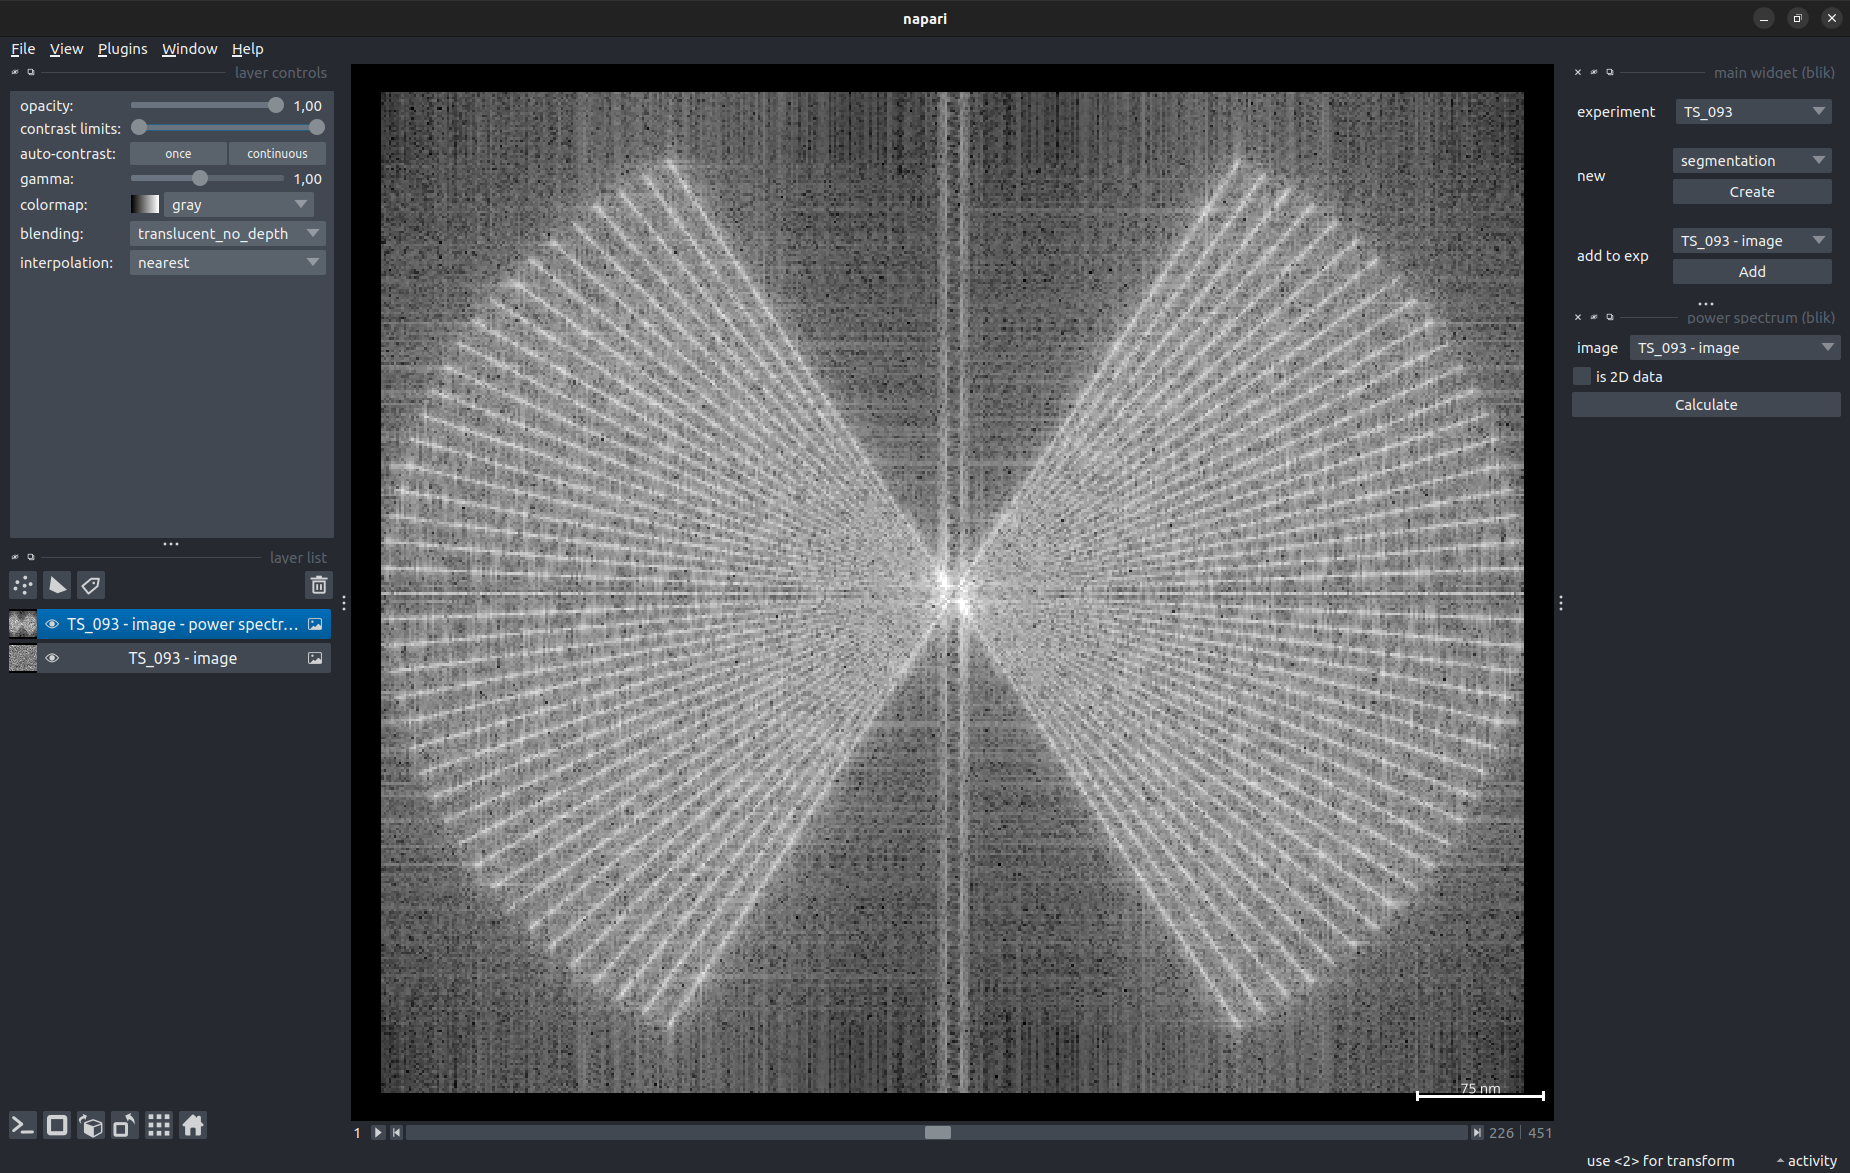
\includegraphics[width=\textwidth]{introduction/missing_wedge.png}
    \titledcaption[Missing wedge]{2D slice through the 3D FT of a tomogram, perpendicular to the tilt axis. The 2D FT of images of the tiltseries are visible as lines at regular angular spacing; at the top and bottom they are not present, creating the missing wedge.}
    \label{fig:et_missing_wedge}
\end{figure}

The high contrast artifacts and information void caused by the missing wedge can make visualisation and annotation of the data difficult.
For this reason, tools have been developed that are able to "fill in" the missing information, improving the visual quality of the tomograms~\cite{liuIsotropicReconstructionElectron2021,zhangMethodRestoringSignals2023}.
While such tools may drastically improve the experience when visualising or annotating data, it's important to not over-interpret the outputs or use them for later steps, lest introducing generated data into the processing.

\section{Annotation and segmentation}\label{et_annotation_segmentation}
Thanks to the \textit{in situ} and quasi-native nature of tomography data, it is often useful to annotate or segment tomograms in order to get a better view of the morphology of the sample, or to find areas and particles of interest more easily.

One of the most common approaches is to do semantic segmentation (aka labeling), where individual voxels are assigned a type --- "membrane", "ribosome", and so on, though usually in the form of a integer --- either by manually painting over the sample, or automatically via image processing algorithms or ML tools.
Labeling helps with visualisation by boiling down the sample to its most fundamental components, while also serving as a powerful tool for quantitative and morphological analysis of complex mesoscale objects.
To this end, segmentations are often used as starting point for other kinds of annotations, such as abstracting membranes or filaments to mathematical objects like splines and skeletons (CITE skan?) in order to calculate properties such as membrane curvature, filament branch length, and so on.

In some projects, morphology is all that matters, with no need to reach high resolution; in such cases, the cryo-ET pipeline can stop after annotation.
Where high resolution molecular structures are the goal, segmentations and other annotations may also be used as a starting point for particle picking.

\section{Particle picking}\label{et_particle_picking}
Picking particles in tomograms is not so different from picking particles from 2D micrographs, other than having an extra dimension.
Manual picking and template matching are still the preferred methods, though more and more software is developed for ML-based or hybrid methods~\cite{wagnerSPHIREcrYOLOFastAccurate2019,wagnerEvolutionSPHIREcrYOLOParticle2020,riceTomoTwinGeneralized3D2023,liuDeepETPickerFastAccurate2024}.

As with most things in cryo-ET, low SNR is the main obstacle to overcome; this is why some picking tools --- such as the one developed during this thesis (\fullref{blik}) --- attempt to use as much prior knowledge about the system as possible in order to limit the degrees of freedom when searching for particles~\cite{castano-diezDynamoCatalogueGeometrical2017,wagnerEvolutionSPHIREcrYOLOParticle2020,gaifasBlikExtensible3D2024}.

Having a 3rd dimension also contributes to making visualisation and annotation harder: particles and structures don't simply lay on a flat plane, and the user interface in software becomes trickier.
Additionally, the missing wedge constitutes an obstacle to annotation, especially for features that are oriented along the microscope axis.

Whenever possible, segmentation or other kinds of annotation can be used as baseline for particle picking: either by masking areas of interest --- such as picking only inside a certain cellular structure --- or by seeding particle picks based on the annotation geometry --- such as distributing particles on the surface of a membrane.
Such information may also be used to initialize the particle orientation to something self-consistent (e.g: all perpendicular to the membrane); this can affect drastically the initial model generation and subsequent refinement, where 3D rotational search may otherwise not overcome the SNR.

\section{Subtomogram averaging}\label{et_sta}
In cryo-ET, the equivalent to SPA's 2D classificatin and 3D refinement is subtomogram averaging (STA).
The idea at the core is the same: by combining the data from many subvolumes extracted from the tomogram (subtomograms) which contain copies of the same object, the SNR can be drastically improved.
The basic procedure is also very similiar to SPA, only in 3D: subtomograms are extracted from the full reconstructed tomogram based on the positions of the particle picks; then, rounds of cross-correlation and refinement (and/or classification) improve the model until convergence (\fullref{em_classification}).

In recent years, however, the field is moving away from this naive approach where "rigid" subtomograms are extracted from a full 3D reconstruction, in favor of what is sometimes called \textbf{per-particle tilt series}~\cite{himesEmClaritySoftwareHighresolution2018,zivanovBayesianApproachSingleparticle2022,tegunovRealtimeCryoelectronMicroscopy2019,chenCompleteDataProcessing2019}.
Differently from the naive method, subtomograms are reconstructed on-the-fly directly from the 2D data, using spatio-temporally adjusted parameters (such as CTF and tilt-series alignment) at the subtomogram level.
This opens up many avenues for optimization --- such as 3D-CTF correction (\fullref{et_tomo_reconstruction})~\cite{turonovaEfficient3DCTFCorrection2017}, multi-particle refinement~\cite{tegunovMultiparticleCryoEMRefinement2021} or bayesian polishing~\cite{zivanovBayesianApproachSingleparticle2022} --- by allowing the subtomogram reconstruction parameters to be tweaked after the first reconstruction (\fullref{em_refinement}).

A significant obstacle during alignment is caused by the missing wedge; it is such a prominent feature that during cross-correlation, it would normally overpower everything else in the subtomograms.
Because of this, subtomograms would end up being rotationally aligned based on how they are rotated relative to the missing wedge, instead of their relative rotation to each other.
For this reason, missing wedge compensation is a crucial step for the success of STA procedures~\cite{galaz-montoyaAlignmentAlgorithmsPerparticle2016} (CITE more).

\section{Refinement}\label{et_refinement}

TODO: not sure if there's anything else to say here, maybe no need.

\section{Pros and Cons}

Cryo-ET has seen a rapid development in recent years, bringing it to the forefront of structual biology techinques.

By providing a high resolution, \textit{in situ} view of biological systems, it brings insights that other \textit{ex situ} techniques like X-ray crystallography and SPA cannot provide.
At the same time, thanks to STA, cryo-ET is able to bridge the gap with single particle analysis, reaching in some cases sub-nanometer resolution for single particle structures, while maintaining the ability to contextualize such structures within the complex biological system they belong to.

A distinctive strength of cryo-ET is the ability to explore mesoscale systems or superstructures --- such as folded 2D lattices and filaments --- without trivializing them for bottom up, \textit{in vitro} reconstitution, and instead observing their structural arrangement as it behaves \textit{in situ}.

Many of cryo-ET's limitations are ultimately ascribable to the low SNR; some of them can be overcome with hardware improvements (better sample preparation, detectors and phase plates), and others with software advances (chromatic aberration correction, better alignment and refinement procedures).
In recent years, several groups are working on developing new hardware and software for cryo-EM and cryo-ET, steadily improving the attainable resolution (\autoref{fig:et_smallest_particle})~\cite{russoCryomicroscopySituWhat2022}.

\begin{figure}[ht]
    \centering
    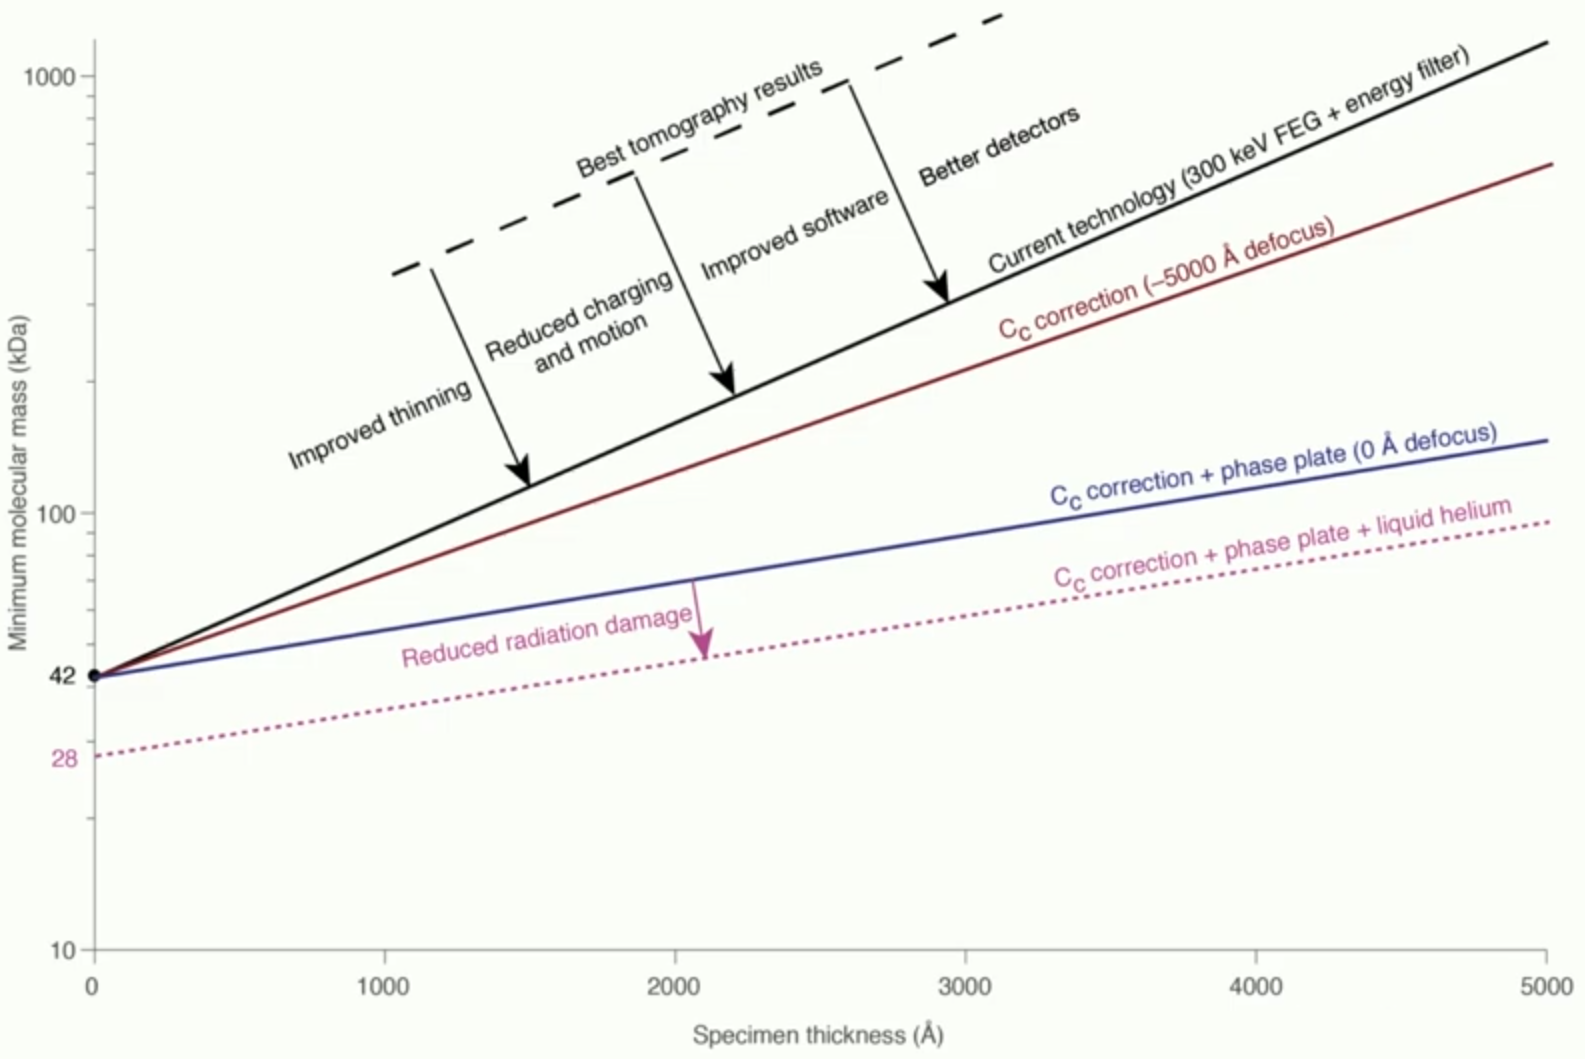
\includegraphics[width=\textwidth]{introduction/smallest_particle_plot_russo.png}
    \titledcaption[Particle size limit versus sample thickness]{Theoretical lower limit of particle size that can be resolved from cryo-EM data, depending on the sample thickness. Currently, even the best tomography results are far from the theoretical limits due to lack of optimization in sample preparation and hardware. The current theoretical limits can yet be improved by implementing some additional methods. Figure taken from \citet{russoElectronCryomicroscopeHardware2023}.}
    \label{fig:et_smallest_particle}
    % TODO: find better version? Ask chris?
\end{figure}

Another common hurdle, especially for researchers new to cryo-ET or programming, is presented by the budding, messy and fragmented software ecosystem. 
